\documentclass[11pt, a4paper]{article}
\usepackage[ a4paper,left = 22mm, right=22mm,
	top=1.3cm, bottom=2cm,
	includehead, includefoot,
	headheight=3 cm]{geometry}
\usepackage[ngerman]{babel}
\usepackage[T1]{fontenc}
\usepackage[utf8]{inputenc}
\usepackage[dvips]{graphicx}
\usepackage{calc}
\usepackage{makeidx}
\usepackage{xcolor}
\usepackage{amsmath,amssymb}
\usepackage{subcaption}
\usepackage{hyperref}
\usepackage{multirow}
\usepackage{fancyhdr}
\usepackage{enumitem}
\usepackage{lastpage}
\usepackage{sectsty}
\usepackage{multirow}

\usepackage{titlesec}
\usepackage{enumitem}
\usepackage{titletoc}
\usepackage{amsmath}
\usepackage{pdfpages}
\usepackage{booktabs}
\usepackage{blindtext}


\usepackage[most]{tcolorbox}




\PackageWarningNoLine{multirow}{warning text}


\allsectionsfont{\sffamily}
\usepackage{eso-pic}
\newcommand\BackgroundWave{%
	\put(0,0){%
		\parbox[b][\paperheight]{\paperwidth}{\vfill \centering \vspace{12.0cm}
			
\includegraphics[width=\paperwidth]{logo/hsel-welle-grey}\vfill }}}%%
\begin{document}
\AddToShipoutPicture{\BackgroundWave}
\begin{titlepage}

\hspace{-1.0cm}
% \hspace{-2.0cm}
\begin{tabular}{p{8.0cm} p{8.0cm}}
  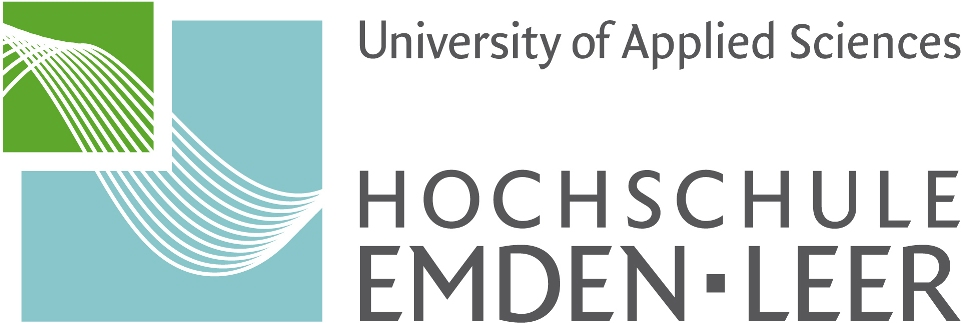
\includegraphics[width = 6.0cm]{img/Technik.png} &
   \parbox[b]{8.0cm}{
     {\large 	Fachbereich Technik }\\
     {\large 	Abteilung Elektrotechnik und Informatik }     
    } \\
   \\
   \hline
\end{tabular}
%
\begin{center}

\vspace{2.5cm}
\LARGE{\textsc{Formelsammlung Elektrotechnik}}\\

\vspace{2cm}%
\large
Oliver Schmidt\hspace{2cm} Matr. Nr. 7023462

\vspace{1cm} 
Emden, \today


\end{center}
\normalsize
\end{titlepage}

\newpage
\pagestyle{fancy}
\fancyhead[L]{{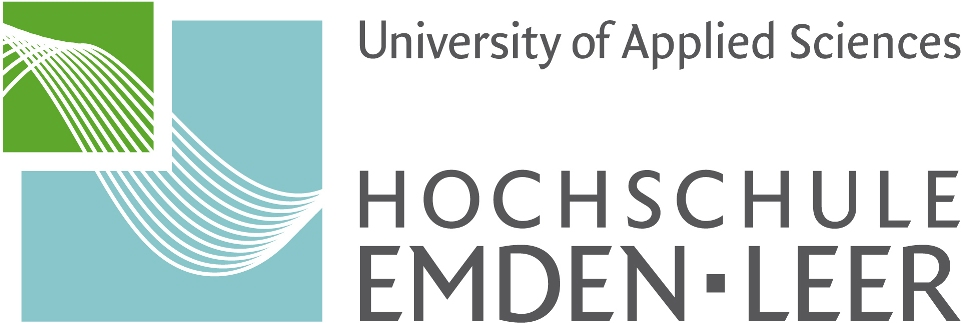
\includegraphics[width = 6.0cm]{img/Technik.png}}}
\fancyhead[R]{
	\Large{{
				Formelsammlung\\
				}}}
\fancyfoot[L]{\rightmark}
\fancyfoot[R]{Seite \thepage\ von \pageref{LastPage}}
\fancyfoot[C]{}
\renewcommand{\footrulewidth}{0.4pt}% Default \footrulewidth is 0pt

\pagenumbering{Roman}
\tableofcontents
\newpage
\listoffigures
\addcontentsline{toc}{section}{Abbildungsverzeichnis}
\newpage
\listoftables
\addcontentsline{toc}{section}{Tabellenverzeichnis}
\newpage
\ClearShipoutPicture

\pagenumbering{arabic}
\section{Magnetisches Feld}
\subsection{Moodle-Übung}
\begin{enumerate}
  \item Magnetische Kraft zwischen zwei parallel verlaufenden, stromdurchflossenen geraden Leitern wobei $a >> d$
        \begin{figure}[h!]
          \begin{center}
            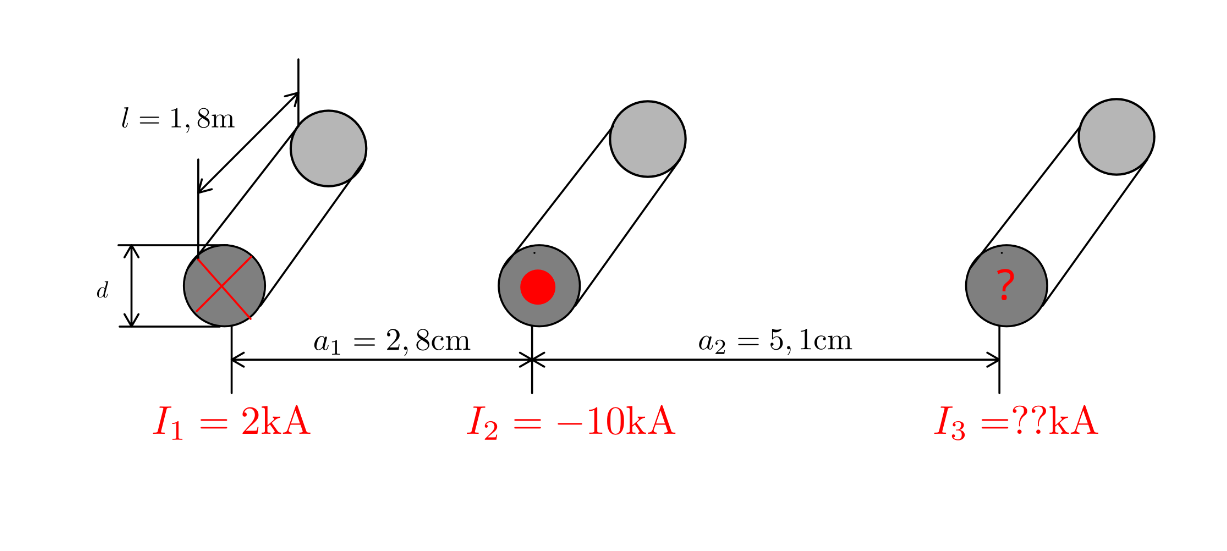
\includegraphics[width=0.75\textwidth]{img/Magnetisches-Feld/A1.png}
          \end{center}
          \caption{Moodle-Übung magnetisches Feld – Kraftwirkung auf drei Leitern}
        \end{figure}
        \begin{align*}
          F_{12}             & = \frac{\mu}{2\pi}\cdot \frac{I_1\cdot I_2}{a}\cdot l                                 \\
          \text{Für } F_{12} & = F_{32} \text{ dann gilt:}                                                           \\
          I_3                & = \frac{I_1\cdot a_2}{a1}                                                             \\
                             & = \frac{2\cdot 10^{3}\text{A}\cdot 5,1\cdot 10^{-2}\text{m}}{2,8\cdot 10^{3}\text{m}} \\
                             & = 3,64\text{kA}                                                                       \\
        \end{align*}

        \begin{align*}
          F_{13} & =\frac{\mu\cdot\mu_{0}}{2\pi}\cdot\frac{I_{1}\cdot I_{3}}{a}\cdot l                                                                                                                         \\
                 & =\frac{4\pi\cdot 10^{-7}\frac{\text{H}}{\text{m}}}{2\pi}\cdot\frac{2\cdot 10^{3}\text{A}\cdot(-10\cdot 10^{-2}\text{A})}{2,8\cdot 10^{3}\text{m}+5,1\cdot 10^{-2}\text{m}}\cdot 1,8\text{m} \\
                 & =-33,202\text{N}                                                                                                                                                                            \\
                 & \Rightarrow |33,20\text{N}|                                                                                                                                                                 \\
        \end{align*}

        \begin{align*}
          F_{23} & =\frac{\mu\cdot\mu_{0}}{2\pi}\cdot\frac{I_{2}\cdot I_{3}}{a}\cdot l                                                                                                                         \\
                 & =\frac{4\pi\cdot 10^{-7}\frac{\text{H}}{\text{m}}}{2\pi}\cdot\frac{2\cdot 10^{3}\text{A}\cdot(-10\cdot 10^{-2}\text{A})}{2,8\cdot 10^{3}\text{m}+5,1\cdot 10^{-2}\text{m}}\cdot 1,8\text{m} \\
                 & =-33,202\text{N}                                                                                                                                                                            \\
                 & \Rightarrow |33,20\text{N}|                                                                                                                                                                 \\
        \end{align*}



        sudo cpan Unicode::GCString
        sudo cpan App::cpanminus
        sudo cpan YAML::Tiny
        sudo perl -MCPAN -e 'install "File::HomeDir"'


\end{enumerate}

\newpage
\section{Elektrische Energietechnik}

\subsection{Thermische Kraftwerke}
\textbf{Wichtige Einheiten und Formelzeichen}:
\newpage
\section{Wechselstromlehre}


\end{document}
